\chapter{Preparation}


\section{Design of a Ring Resonator}
\label{design}
To filter a special wavelength using a ring resonator the design of the resonator needs to be adjusted to the wavelength.
\begin{figure}[h]%
\centering
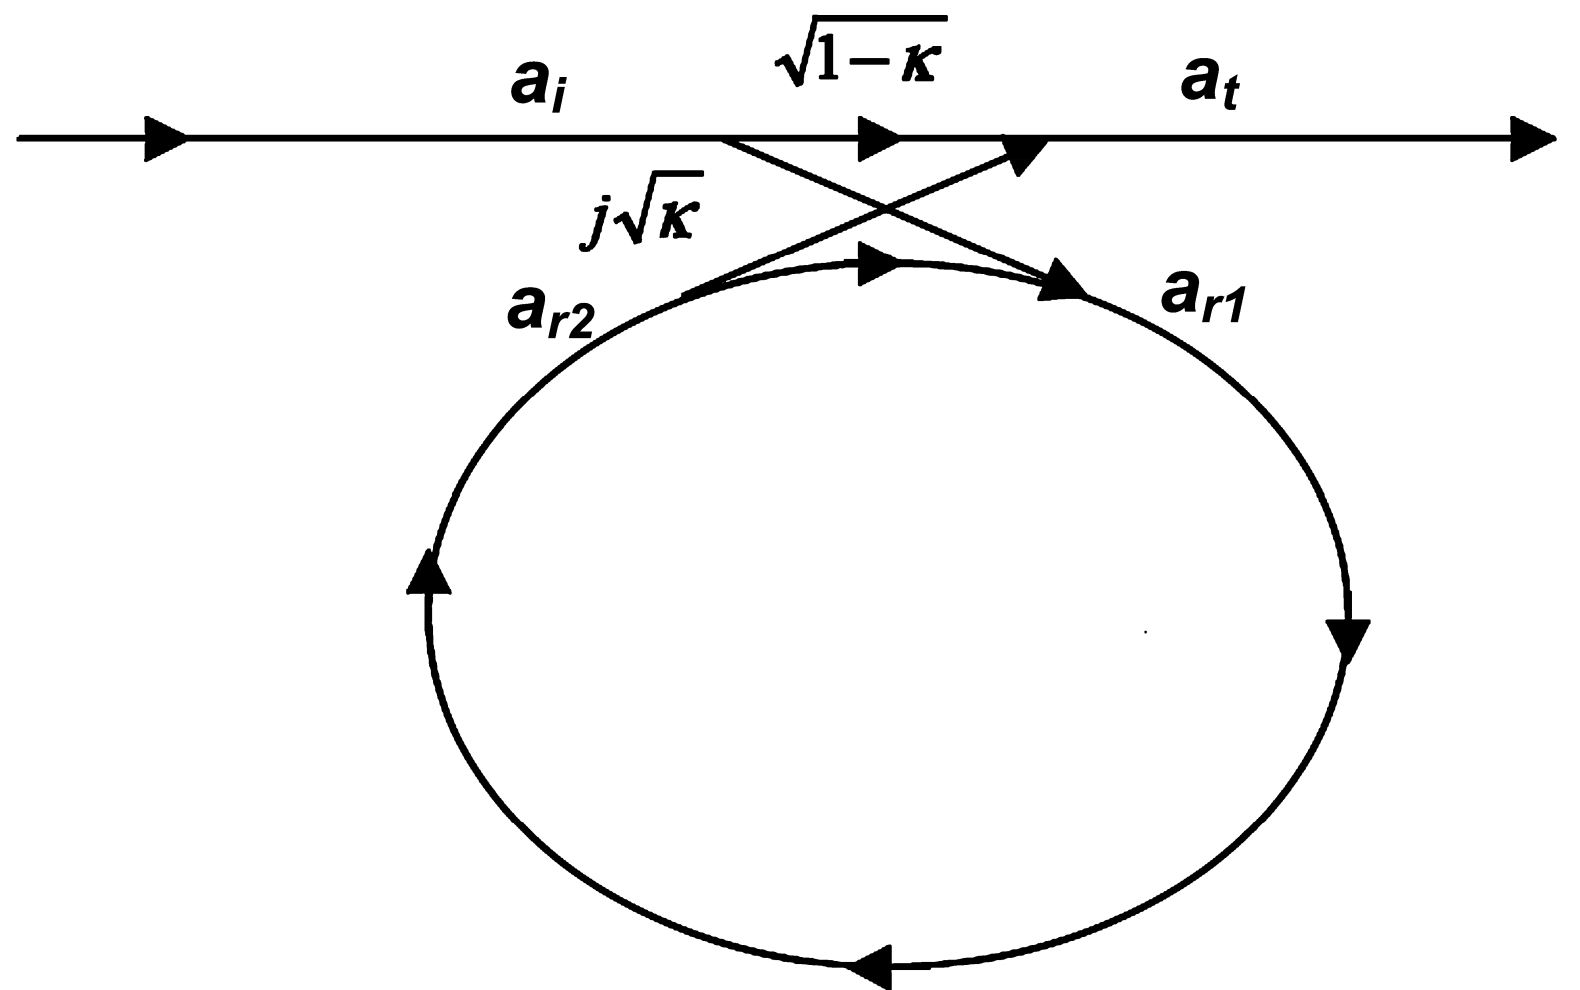
\includegraphics[width=.5\columnwidth]{Grafiken/Resonator.png}%
\caption{Schematic of a ring resonator.}%
\label{fig:p1_ring}%
\end{figure} 
Figure \ref{fig:p1_ring}\footnote[1]{Jingshi Li, Materials for the preparation of Experiment 6} shows a schematic picture of a parallel ring resonator. It consists of a coupling zone between the ring resonator and the waveguide which can be modeled as directional coupler\footnotemark[1].

The transmission of the ring follows the relation:

\begin{equation}
a\i{r2}=a_{\mathrm{r1}}\cdot e^{-\alpha /2\cdot L}\cdot e^{-j\beta L}
\label{eq:}
\end{equation}
That means the ring is in resonance
\begin{equation}
\beta L = m\cdot2\pi,\qquad m \in \mathbf{N}
\label{eq:res}
\end{equation}
wiht $\beta = n_{\mathrm{eff}} \frac{2\pi f}{c} = n_{\mathrm{eff}} \frac{2\pi}{\lambda_0}$.

Using the transmission of the ring and the matrix of the directional coupler a term for the transmitted power can be derived\footnotemark[1]:
\begin{equation}
T(\beta L) = \frac{|a_t|^2}{|a_i|^2}= \frac{(1-e^{-\alpha \cdot L})(1-(1-\kappa))}{(1-e^{-\alpha /2\cdot L}\sqrt{1-\kappa})^2+4e^{-\alpha /2\cdot L}\sqrt{1-\kappa}\cdot\mathrm{sin}^2(\beta L / 2)}
\label{eq:}
\end{equation}
As described above the ring is in resonance for $\beta L = m\cdot2\pi$ and the transmission becomes minimum. 
In this case
\begin{equation}
T_{\mathrm{min}}=\frac{(e^{-\alpha /2\cdot L} - \sqrt{1-\kappa})^2}{(1 - e^{-\alpha /2\cdot L}\sqrt{1-\kappa})^2}
\label{eq:}
\end{equation}

When $e^{-\alpha /2\cdot L} = \sqrt{1-\kappa}$ the transmission is zero. This case is called $critical~coupling$ and can be achieved for 
\begin{equation}
\alpha = - \frac{1}{L}\mathrm{ln}(1-\kappa)\quad .
\label{eq:crti}
\end{equation}


To design ring resonator filter to block certain wavelength there are different approaches.
At first the filter could consist of different in series connected parallel ring resonators. Each resonator would filter characteristic frequencies.
For the given wavelength $\lambda_1 = 1550$~nm and $\lambda_2 = 1551$~nm some other approaches are conceivable.

Secondly one resonator could be used with a resonance frequency between $\lambda_1$ and $\lambda_2$. If the width of the resonance line is broader than than the difference between $\lambda_1$ and $\lambda_2$ both wavelengths get filtered.

Further the design of the waveguide used for the ring resonator (material, dimensions) could be chosen, that the effective indices for the two waveguides are just so that 

\begin{equation}
\frac{2\pi n_{\mathrm{eff,1}}}{\lambda_1} = \frac{2\pi n_{\mathrm{eff,2}}}{\lambda_2}
\label{eq:}
\end{equation}
is true.

Finally there is the possibility to adjust the size of ring resonator. The Free Spectral Range that describes the distance between two resonances $m$ and $m+1$ is approximately

\begin{equation}
\Delta f \approx \frac{c}{n\i{g}\cdot L}
\label{eq:abstand}
\end{equation}

Calculating $\Delta f$ for the given values:

\begin{equation}
|\Delta f| = \left|-\frac{c}{\lambda^2}\Delta\lambda\right| =~125~\mathrm{GHz}.
\label{eq:}
\end{equation}

This leads to 

\begin{equation}
L \approx \frac{3\cdot10^8}{n\i{g}\cdot125\cdot10^9}=\frac{2.40\cdot10^{-3}}{n\i{g}}
\label{eq:}
\end{equation}

For a ring resonator with this length the neighbouring dips have a distance of $\sim1$~nm. So with one Resonator two dips at the example wavelength could be realized.

\section{Measuring the Resonator Parameters}

\begin{figure}[h]%
\centering
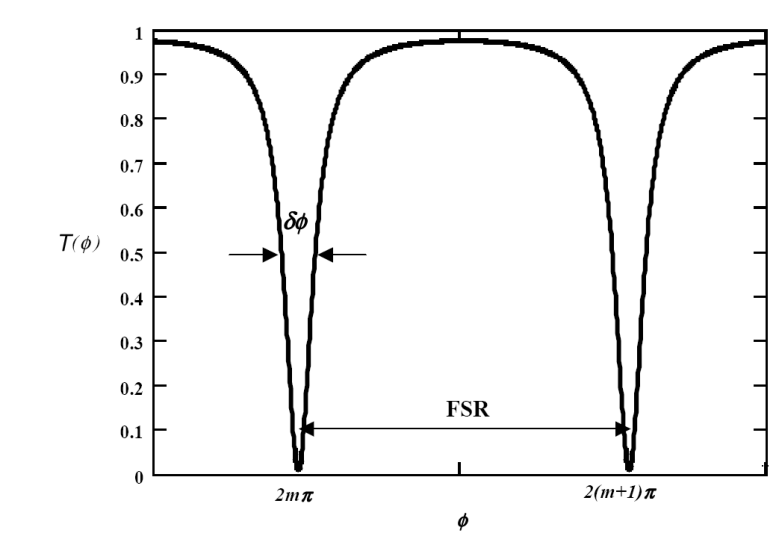
\includegraphics[width=.5\columnwidth]{Grafiken/S21.pdf}%
\caption{Example Transmission Coefficient of a Resonator}%
\label{fig:S21}%
\end{figure}

To characterize a resonator its power transmission in dependency of the frequency can easily be measured. By that measurement, the width of the resonance lines at full width half maximum (FWHM) $\delta f$ and the free spectral range $\Delta f$ can determined. (cf. figure \ref{fig:S21}). The quotient $F= \Delta f/\delta f$ is called Finesse. For the case of critical coupling $F$ is given as:
\begin{equation}
 F = \frac{\Delta f}{\delta f} = \frac{\pi\sqrt{1-\kappa}}{\kappa}=\frac{\pi\exp\left(-\alpha L/2\right)}{1-\exp\left(-\alpha L\right)}
\end{equation}
This can be rearranged to:
\begin{equation}
 \kappa = \frac{-\pi^2 \pm \sqrt{\pi^4+4F^2\pi^2}}{2F^2}
 \label{eq:kappa}
\end{equation}
and
\begin{equation}
\alpha = \frac{2\ln\frac{\sqrt{4F^2+\pi^2}+\pi}{2F}}{L} 
\label{eq:alpha}
\end{equation}
respectively.

\section{Over-Critical and Under-Critical coupling}
\begin{figure}[h]%
\centering
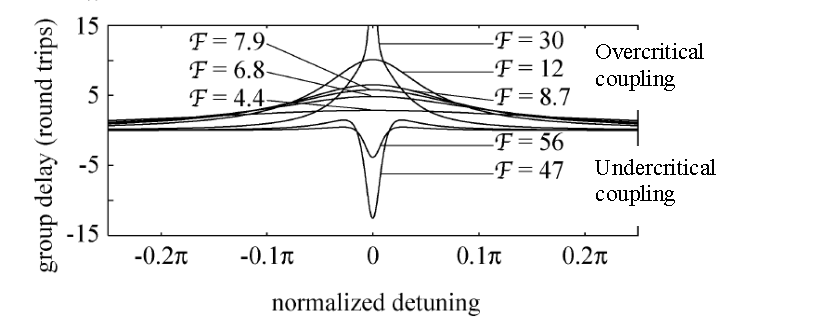
\includegraphics[width=.7\columnwidth]{Grafiken/crit_coupling.pdf}%
\caption{group delay in dependency of the detuning for different Finesses}%
\label{fig:crit_coupling}%
\end{figure}

For over and undercritical coupling the group delay changes at the resonance frequency. This behavior can be seen in figure \ref{fig:crit_coupling}. For overcritical coupling the losses in the ring are smaller than the coupling losses. The signal gets delayed, so the group delay is positive. For undercritical damping the losses in the ring are greater than the coupling losses. In this case the group velocity becomes negative.

The design of a filter with a over or undercoupled system is disadvantageous. The ideal case is critical damping. There the part that is directly transmitted from the input to the output is extinguished by the part that couples out of the resonator. In the case of undercritical coupling the wave needs some circulations in the resonator till it vanishes. Each time it passes the coupler, the wave is coupled to the output. The signal from the input is depleted by the first circulation, thus each additional circulation couples energy to the output.
In the case of overcritical coupling the wave is depleted within one circulation. Thus there is no wave that is coupled out of the resonator, that depletes the wave coupled from the input to the output.
In both cases, overcritical and undercritical coupling, the Quality $Q$ is decreased.
